\documentclass[12pt]{article}

\usepackage[english]{babel}
\usepackage[utf8x]{inputenc}
\usepackage{amsmath}
\usepackage{graphicx}
\usepackage{ulem}
\usepackage[colorinlistoftodos]{todonotes}
\usepackage{listings}
\usepackage{glossaries}
\usepackage[
top    = 2.75cm,
bottom = 2.00cm,
left   = 2.50cm,
right  = 2.00cm]{geometry}
\setcounter{secnumdepth}{4}

\makeglossaries

\newglossaryentry{er} {name=ER, description={Entity Relation}}
\newglossaryentry{ddl} {name=DDL, description={Data Definition Language}}
\newglossaryentry{sql} {name=SQL, description={Structured Query Language}}

\begin{document}
\begin{titlepage}
\begin{center}
% Oberer Teil der Titelseite:

\includegraphics[width=0.5\textwidth]{images/logo}\\[1cm]    

\textsc{\LARGE Technisches Gewerbe Museum}\\[1.5cm]

% Title
\rule{12cm}{1mm}
{ \huge \bfseries  \\\large DEZSY\\ \huge Distributed Databases \\[0.4cm] }

\rule{12cm}{1mm}

% Author and supervisor
\noindent 
\vspace{5cm}

\begin{center}
\large
Author: 
Ahmed \textsc{Aly} \&
Hannah \textsc{Siegel}
\end{center}

\vfill

% Bottom of the page
{\large \today}

\end{center}
\end{titlepage}

\tableofcontents

\newpage

\section{Task description}
\label{sec:aufgabenstellung}
The Task description can be found under:

\section{Working time}
\subsection{Estimated working time}
\begin{table}[h]
\begin{tabular}{|p{0.6\textwidth}|p{0.2\textwidth}|p{0.2\textwidth}|}
\hline
\textbf{Task}    & \textbf{Person}                                               & \textbf{Time in hours                              } \\ \hline \hline
\gls{er}-diagram & \begin{tabular}[c]{c}Aly\\ Siegel\end{tabular} & \begin{tabular}[c]{c}1\\ 3\end{tabular}   \\ \hline
\gls{ddl} & \begin{tabular}[c]{c}Aly\\ Siegel\end{tabular} & \begin{tabular}[c]{c}1\\3\end{tabular}   \\ \hline
\gls{sql} & \begin{tabular}[c]{c}Aly\\ Siegel\end{tabular} & \begin{tabular}[c]{c}1\\2\end{tabular}   \\ \hline
Installation and Setup of OrcaleEX& \begin{tabular}[c]{c}Aly\\ Siegel\end{tabular}&\begin{tabular}[c]{c}3\\ 1\end{tabular}   \\ \hline
Fragmentation & \begin{tabular}[c]{c}Aly\\ Siegel\end{tabular} & \begin{tabular}[c]{c}3\\ 3\end{tabular}   \\ \hline
Testing of some queries & \begin{tabular}[c]{c}Aly\\ Siegel\end{tabular} & \begin{tabular}[c]{c} 2\\ 2\end{tabular}   \\ \hline 
Documentation & \begin{tabular}[c]{c}Aly\\ Siegel\end{tabular} & \begin{tabular}[c]{c} 2\\ 2\end{tabular}   \\ \hline \hline
Total & \begin{tabular}[c]{c}Aly\\ Siegel\end{tabular} & \begin{tabular}[c]{c}13\\16\end{tabular}   \\ \hline 
\textbf{Total Team} & & \textbf{29 hours}  \\ \hline 

\end{tabular}
\end{table}
\subsection{Actual time}
\begin{table}[h]
\begin{tabular}{|p{0.6\textwidth}|p{0.2\textwidth}|p{0.2\textwidth}|}
\hline
\textbf{Task}   & \textbf{Person}     & \textbf{Time in hours  } \\ \hline \hline
\gls{er}-diagram & \begin{tabular}[c]{c}Aly\\ Siegel\end{tabular} & \begin{tabular}[c]{c}3\\ 4\end{tabular}   \\ \hline
\gls{ddl} & \begin{tabular}[c]{c}Aly\\ Siegel\end{tabular} & \begin{tabular}[c]{c}0\\2\end{tabular}   \\ \hline
Installation and Setup of OrcaleEX& \begin{tabular}[c]{c}Aly\\ Siegel\end{tabular}&\begin{tabular}[c]{c}3\\ 1\end{tabular}   \\ \hline
Fragmentation & \begin{tabular}[c]{c}Aly\\ Siegel\end{tabular} & \begin{tabular}[c]{c}2\\ 2\end{tabular}   \\ \hline
Testing of some queries & \begin{tabular}[c]{c}Aly\\ Siegel\end{tabular} & \begin{tabular}[c]{c} 2\\ 2\end{tabular}   \\ \hline 
Documentation & \begin{tabular}[c]{c}Aly\\ Siegel\end{tabular} & \begin{tabular}[c]{c} 2\\ 2\end{tabular}   \\ \hline \hline
Total & \begin{tabular}[c]{c}Aly\\ Siegel\end{tabular} & \begin{tabular}[c]{c}XXX\\XXX\end{tabular}   \\ \hline 
\textbf{Total Team} & & \textbf{XXX hours}  \\ \hline 
\end{tabular}
\end{table}

\section{Theoretical Background}
\section{Implementation}
\subsection{Database-design}
\subsubsection{Understanding the Task}
We copied the task description from section \ref{sec:aufgabenstellung} into an word document. 
Then we were deleting all the superficial information, until we had some sort of inofficial RM: \\
\\
\textbf{Meal}(\underline{ID}, name, type {starter, main\_dish,dessert}) \\
A meal contains a \textit{quantity} of \\
\textbf{Ingredient}(\underline{ID}, name, unit {kg, l} price) \\
\textbf{Cafeteria}  (\underline{ID},name) \\
A cafeteria has vendors  \\
\textbf{Vendor}(\underline{ID}, address) \\
\textbf{Storage} (\underline{ID},\dashuline{Ingredient.ID}, quantity) \\
\textbf{Order}(\underline{ID},\dashuline{Vendor.ID}, date\_ordered, date\_delivered ) \\
\textbf{Orderinclude}(\dashuline{Order.ID},\dashuline{Ingredient.ID}, quantity, price) \\
\textbf{Bill}(\underline{ID}, \dashuline{Order.ID}, IBAN, BIC, total\_sum) \\
\textbf{Menu}(\underline{ID},name,price) \\
\textbf{Day}(\underline{ID}, date, starter, main\_dish, dessert) \\
\subsubsection{ER-Diagram}
We decided to use Astah. We have never used it before and so it was a little bit difficult to get all the relationships right.
In figure \ref{fig:try1} our first database design can be seen.
 \begin{figure}[here!]
	\centering
	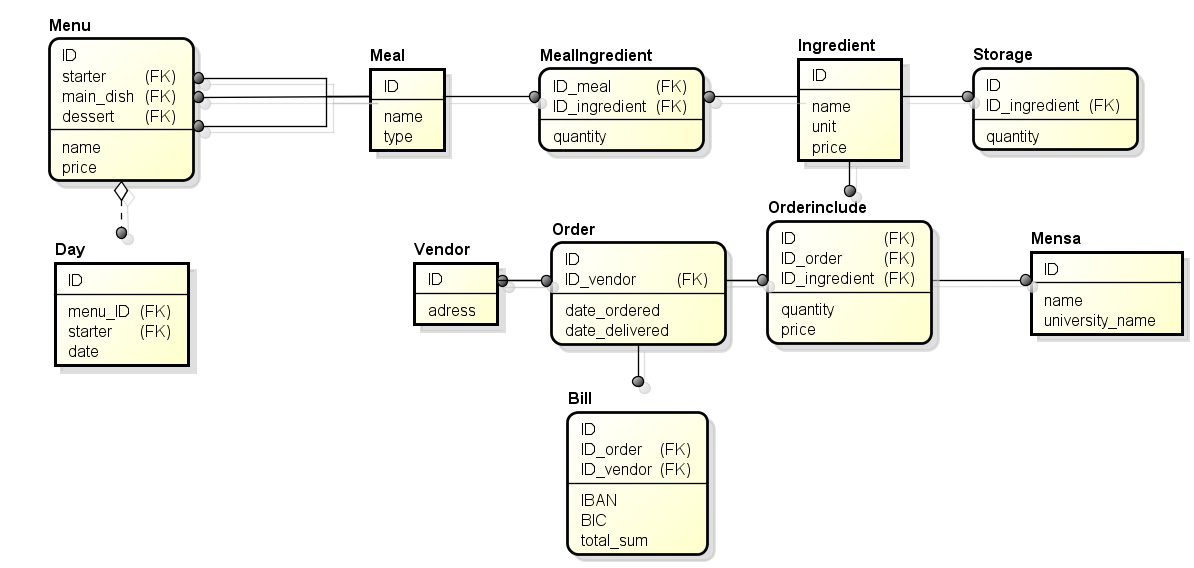
\includegraphics[width=1.0\textwidth]{er_vorlaeufig.png}
	\caption{The first try to make an working ER-Diagram with Astah}
	\label{fig:try1}
	\end{figure}
	
\subsubsection{\gls{ddl}}
Whenever using Astah, it is possible to export the \gls{er}-diagram into an \gls{sql} file. \\
Unfortunately this didn't work out, because we were not able to import the file which has been exported by Astah.
The syntax of the Order table was not right and we were not able to find a solution. The exported file will be in the disposal of this exercise. \\ \\
We then decided to simply code the \gls{ddl} by our selves, because we already know how to do so. It took us a little bit longer because there were some unnecessary faults, like a semicolon missing.

 

	
\newpage
\printglossaries
\listoffigures
\newpage
\begin{thebibliography}{56}

\bibitem{thorstenhorn}
   \textbf{Torsten Horn}\newline
  \emph{http://www.torsten-horn.de/techdocs/eai.htm}
  \newline abgerufen am: 05.10.2014, 20:25


\end{thebibliography}

\end{document}

